\chapter{The Eilenberg-Zilber module}

The functions of this module are related to the chain complex of the
pro\-duct of two simplicial sets.
They implement the Eilenberg-Mac Lane homomorphism (function {\tt eml}) 
and the Alexander-Whitney homomorphism  (function {\tt aw}).
\vskip 0.45cm
{\parindent=0mm
{\leftskip=5mm 
{\tt eml} {\em ssx ssy} \hfill {\em [Function]} \par}
{\leftskip=15mm 
build\index{homomorphism!Eilenberg-Mac Lane} the Eilenberg-Mac Lane homomorphism $\cal EML$, also called 
the {\em shuffle homomorphism}\footnote{{\bf Marvin Greenberg}, {\it Lectures on Algebraic Topology}, 
W.A. Benjamin Inc, 1967.}.
The arguments {\em ssx} and {\em ssy} represent some simplicial sets $X$ and $Y$.
The homomorphism 
$${\cal EML}:{\cal C}_*(X) \otimes {\cal C}_*(Y) \longrightarrow {\cal C}_*(X \times Y)$$
is defined by:
$${\cal EML}(\alpha \otimes \beta)= 
 \sum{{\varepsilon(\varpi)}(\eta_{j_q}\ldots \eta_{j_1}\alpha,\, \eta_{i_p}\ldots \eta_{i_1}\beta)},$$
where $X\times Y$ is the simplicial cartesian product of the two simplicial sets $X$ and $Y$,  $\alpha$ (resp. $\beta$)
is a geometric simplex of $X$ (resp. $Y$), $\eta_k$ is the $k^{th}$ degeneracy operator, the sum is
over all permutations $\varpi= (i_1 \ldots i_p j_1 \ldots j_q)$ of $(0 \ldots p+q-1)$ such that
$$ i_1 < i_2 < \cdots < i_p,\quad j_1 < j_2 < \cdots < j_q, \quad p+q=n$$
and $\varepsilon(\varpi)$ is the signature of the corresponding permutation. The sum at the right hand part determines
a decomposition of the geometric product $\alpha \times \beta$ into a combination of generators of the
simplicial cartesian product (see the simplicial sets chapter). The combination takes in account the orientation of every
simplex. These generators are non-degenerate simplices of the cartesian product but their projections 
are in general degenerate simplices of $X$ and $Y$ (see the examples). \par}
{\leftskip=5mm 
{\tt aw} {\em ssx ssy} \hfill {\em [Function]} \par}
{\leftskip=15mm 
build\index{homomorphism!Alexander-Whitney} the Alexander-Whitney chain homomorphism.
The arguments {\em ssx} and {\em ssy} represent some simplicial sets $X$ and $Y$.
The homomorphism 
$${\cal AW}:{\cal C}_*(X \times Y) \longrightarrow {\cal C}_*(X) \otimes {\cal C}_*(Y)$$
is defined by the following rule: let $\sigma$ be an $n$-simplex and let us define
two operators, $\lambda_p$ and $\rho_q$:
$$\lambda_p: {\cal C}_n(X) \longrightarrow {\cal C}_{n-p}(X),\quad (n \geq p),$$
$$\rho_q: {\cal C}_n(Y) \longrightarrow {\cal C}_{n-q}(X),\quad (n \geq q),$$
respectively by
$$\lambda_p(\sigma)=\partial_{p+1}\ldots \partial_n \sigma$$
and
$$\rho_q(\sigma)=\partial_0\ldots\partial_{n-q} \sigma.$$
Now, for the generator $(\alpha,\beta)$  of degree $n$ in ${\cal C}_*(X \times Y)$, the Alexander-Whitney homomorphism
is defined  by:
$${\cal AW}(\alpha, \beta)=\sum_{p=0}^n{\lambda_p(\alpha) \otimes \rho_{n-p}(\beta)}.$$
This sum can be interpreted as a decomposition, up to a homotopy, of the simplex $\alpha \times \beta$
($\alpha$ {\bf and} $\beta$ can be degenerate even if $\alpha \times \beta$ is not) in terms of (tensor)
products of non-degenerate simplices.
\par}
{\leftskip=5mm 
{\tt phi} {\em ssx ssy} \hfill {\em [Function]} \par}
{\leftskip=15mm 
build the homotopy chain morphism 
$$\Phi: {\cal C}_*(X \times Y) \longrightarrow {\cal C}_*(X \times Y)$$
satisfying the formula
$$d \circ \Phi + \Phi \circ d = Id - {\cal EML} \circ {\cal AW}.$$
\par}
}
\newpage
{\parindent=0mm
{\leftskip=5mm 
{\tt ez} {\em ssx ssy}  \hfill {\em [Function]} \par}
{\leftskip=15mm 
build the Eilenberg--Zilber reduction as shown by the following dia\-gram, where $X={\mathit ssx}$ 
and $Y={\mathit ssy}$.
$$
\diagram{
{{\cal C}_*(X \times Y)} & \stackrel{\Phi}{\longrightarrow} & {}^s{{\cal C}_*(X \times Y)} \cr
 {\scriptstyle {\cal AW}} \downarrow \uparrow {\scriptstyle {\cal EML}}  \cr
 {{\cal C}_*(X) \otimes {\cal C}_*(Y)} \cr
}
$$
\par}}
\begin{center}
-------------
\end{center}
\newpage

\subsection* {Examples}
%
\vskip 0.40cm
\centerline{\includegraphics{eml1.eps}}
\vskip 0.40cm
%
As simplicial sets $X$ and $Y$, let us use two copies of $\Delta^{\N}$, that we may build
by the lisp statement {\tt (soft-delta-infinity)} (Though we repeat this statement
in the following line, there will be only a simplicial set created). We have chosen the {\em soft}
version, to inspect  the results more easily. 
{\footnotesize\begin{verbatim} 
(setf eml-mrp (eml (soft-delta-infinity)(soft-delta-infinity)))  ==>

[K11 Morphism (degree 0)]
\end{verbatim}}
Let us apply the Eilenberg-Mac Lane homomorphism to the tensor product
$(0\, 1)\otimes (2\, 3)$:
{\footnotesize\begin{verbatim} 
(? eml-mrp 2 (tnpr 1 (d(dlop-ext-int '(0 1)))
                   1 (d(dlop-ext-int '(2 3)))))   ==>

----------------------------------------------------------------------{CMBN 2}
<-1 * <CrPr 0 0-1 1 2-3>>
<1 * <CrPr 1 0-1 0 2-3>>
------------------------------------------------------------------------------
\end{verbatim}}
\newpage
The decomposition is illustrated by the previous geometric diagram, where for instance
a degenerate simplex like $\eta_1(0\, 1)$ is noted $(0\, 1\, 1)$.
\par
For the tensor product $(0\,1\,2)\otimes (3\,4)$, an intuitive description
is still possible, as shown in the following diagram, but not in higher dimensions.
\par
As the input of simplices is sometimes cumbersome, we have defined a macro called {\tt code}
to facilitate the input of the simplices.
{\footnotesize\begin{verbatim} 
(defmacro code (arg) `(d (dlop-ext-int ,arg)))  ==>

CODE

(? eml-mrp 3 (tnpr 2 (code '(0 1 2)) 1 (code '(3 4)) ))  ==>

----------------------------------------------------------------------{CMBN 3}
<1 * <CrPr 0 0-1-2 2-1 3-4>>
<-1 * <CrPr 1 0-1-2 2-0 3-4>>
<1 * <CrPr 2 0-1-2 1-0 3-4>>
------------------------------------------------------------------------------

(? eml-mrp 6 (tnpr 2 (code '(0 3 5)) 4 (code '(0 1 2 4 5)) ))  ==>

----------------------------------------------------------------------{CMBN 6}
<1 * <CrPr 3-2-1-0 0-3-5 5-4 0-1-2-4-5>>
<-1 * <CrPr 4-2-1-0 0-3-5 5-3 0-1-2-4-5>>
<1 * <CrPr 4-3-1-0 0-3-5 5-2 0-1-2-4-5>>
<-1 * <CrPr 4-3-2-0 0-3-5 5-1 0-1-2-4-5>>
<1 * <CrPr 4-3-2-1 0-3-5 5-0 0-1-2-4-5>>
<1 * <CrPr 5-2-1-0 0-3-5 4-3 0-1-2-4-5>>
<-1 * <CrPr 5-3-1-0 0-3-5 4-2 0-1-2-4-5>>
<1 * <CrPr 5-3-2-0 0-3-5 4-1 0-1-2-4-5>>
<-1 * <CrPr 5-3-2-1 0-3-5 4-0 0-1-2-4-5>>
<1 * <CrPr 5-4-1-0 0-3-5 3-2 0-1-2-4-5>>
<-1 * <CrPr 5-4-2-0 0-3-5 3-1 0-1-2-4-5>>
<1 * <CrPr 5-4-2-1 0-3-5 3-0 0-1-2-4-5>>
<1 * <CrPr 5-4-3-0 0-3-5 2-1 0-1-2-4-5>>
<-1 * <CrPr 5-4-3-1 0-3-5 2-0 0-1-2-4-5>>
<1 * <CrPr 5-4-3-2 0-3-5 1-0 0-1-2-4-5>>
------------------------------------------------------------------------------
\end{verbatim}}
\newpage
%
\vskip 0.40cm
\centerline{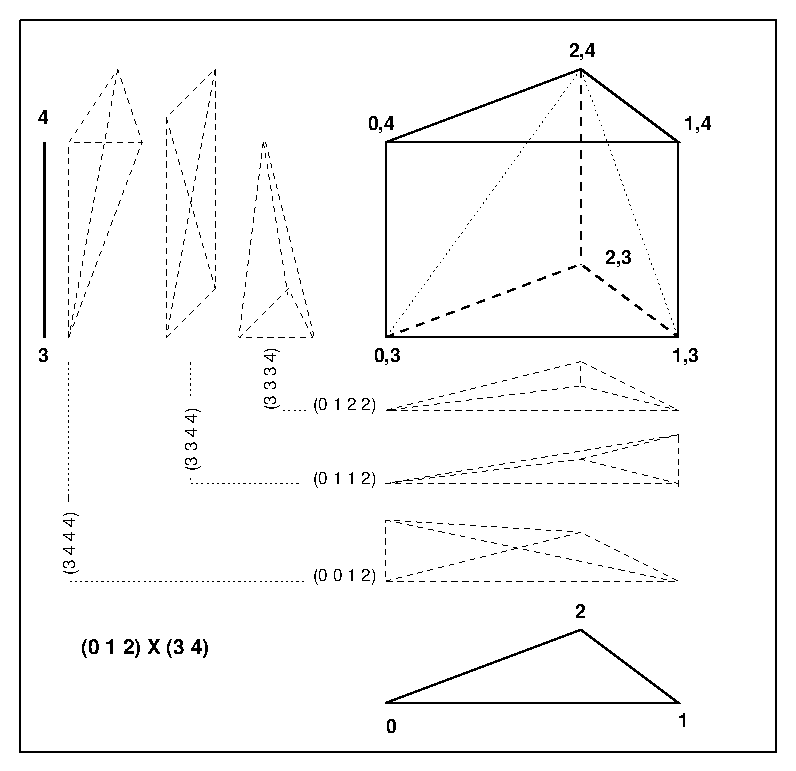
\includegraphics{eml2.eps}}
\vskip 0.40cm
%

The Alexander-Whitney homomorphism works in the reverse sense:
{\footnotesize\begin{verbatim}
(setf aw-mrp (aw (soft-delta-infinity)(soft-delta-infinity)))  ==>

[K12 Morphism (degree 0)]
\end{verbatim}}
The 2-simplices of the cartesian product $(0\, 1\, 2) \times (3\, 4)$ are (here, the degeneracy
operators are in clear):
{\footnotesize\begin{verbatim}
      <CrPr 0 (0 1) 1 (3 4)>
      <CrPr 1 (0 1) 0 (3 4)>
      <CrPr 0 (0 2) 1 (3 4)>
      <CrPr 1 (0 2) 0 (3 4)>
      <CrPr 0 (1 2) 1 (3 4)>
      <CrPr 1 (1 2) 0 (3 4)>
      <CrPr * (0 1 2) 1-0 (3)>
      <CrPr * (0 1 2) 1-0 (4)>
 -->  <CrPr * (0 1 2) 0 (3 4)>
      <CrPr * (0 1 2) 1 (3 4)>
\end{verbatim}}
The last but one line of this list describes the triangle shown in dashed lines in the prism
in the previous picture, joining the points $(0,3), (1,3), (2,4)$. 
Let us apply  the homomorphism $\cal AW$:
{\footnotesize\begin{verbatim}
(? aw-mrp 2 (crpr 0 (code '(0 1 2)) 1 (code '(3 4)) ))  ==>

----------------------------------------------------------------------{CMBN 2}
<1 * <TnPr 0-1 3-4>>
<1 * <TnPr 0-1-2 4>>
------------------------------------------------------------------------------
\end{verbatim}}
We see that we obtain  a kind of decomposition, up to a homotopy, of this triangle
in terms of the two tensor products $(0\, 1\, 2) \otimes (4)$ (the ``upper'' triangle of
the prism) and $(0\,1) \otimes (3\, 4)$ (the ``front'' rectangle of the prism).
\par
\medskip
The composition ${\cal AW} \circ {\cal EML}$ is the identity in the tensor product of
the two chain complexes.
{\footnotesize\begin{verbatim}
(setf g (tnpr 2 (code '(0 1 2)) 3 (code '(2 3 4 5)) ))  ==>

<TnPr 0-1-2 2-3-4-5>

(? eml-mrp 5 g)  ==>

----------------------------------------------------------------------{CMBN 5}
<1 * <CrPr 2-1-0 0-1-2 4-3 2-3-4-5>>
<-1 * <CrPr 3-1-0 0-1-2 4-2 2-3-4-5>>
<1 * <CrPr 3-2-0 0-1-2 4-1 2-3-4-5>>
<-1 * <CrPr 3-2-1 0-1-2 4-0 2-3-4-5>>
<1 * <CrPr 4-1-0 0-1-2 3-2 2-3-4-5>>
<-1 * <CrPr 4-2-0 0-1-2 3-1 2-3-4-5>>
<1 * <CrPr 4-2-1 0-1-2 3-0 2-3-4-5>>
<1 * <CrPr 4-3-0 0-1-2 2-1 2-3-4-5>>
<-1 * <CrPr 4-3-1 0-1-2 2-0 2-3-4-5>>
<1 * <CrPr 4-3-2 0-1-2 1-0 2-3-4-5>>
------------------------------------------------------------------------------

(? aw-mrp *)

----------------------------------------------------------------------{CMBN 5}
<1 * <TnPr 0-1-2 2-3-4-5>>
------------------------------------------------------------------------------

(setf *tnpr-with-degrees* t)  ==>

T

**

----------------------------------------------------------------------{CMBN 5}
<1 * <TnPr 2 0-1-2 3 2-3-4-5>>
------------------------------------------------------------------------------
\end{verbatim}}
But the composition ${\cal EML} \circ {\cal AW}$ is by no means the identity. This composition
is related to the identity via the homotopy morphism $\Phi$. Let us consider the
two following simple simplicial sets {\tt delta-0-1} and {\tt delta-2-3}, where the
second is the simplicial set, model of the segment $[2,\,3]$. To build {\tt delta-2-3}, we
have just changed the basis function, the base point and the comment in the system function {\tt soft-delta}.
{\footnotesize\begin{verbatim}
(setf delta-0-1 (soft-delta 1))

[K13 Simplicial-Set]

(setf delta-2-3 (build-smst 
                  :cmpr #'soft-delta-cmpr
                  :basis #'(lambda(dmn) 
                             (case dmn
                                  (0 (list (d 4)(d 8)))
                                  (1 (list(d 12)))))   
                  :bspn (d 4)
                  :face #'soft-delta-face
                  :intr-dgnl #'soft-delta-dgnl :dgnl-strt :gnrt
                  :intr-bndr #'soft-delta-bndr :bndr-strt :gnrt
                  :orgn '(my-soft-delta-2-3)))

[K18 Simplicial-Set]

(show-structure delta-0-1 1)  ==>

Dimension = 0 :

        Vertices :  (0 1)

Dimension = 1 :

        Simplex : 0-1

                Faces : (<AbSm - 1> <AbSm - 0>)

(show-structure delta-2-3 1)  ==>

Dimension = 0 :

        Vertices :  (2 3)

Dimension = 1 :

        Simplex : 2-3

                Faces : (<AbSm - 3> <AbSm - 2>)
\end{verbatim}}
Let us build the cartesian product of these two simplicial sets and let us list,
in particular the 
0-simplices and the 1-simplices of this new simplicial set:
{\footnotesize\begin{verbatim}
(setf carre (crts-prdc delta-0-1 delta-2-3))  ==>

[K23 Simplicial-Set]

(show-structure carre 2)  ==>


Dimension = 0 :

        Vertices :  (<CrPr - 0 - 2> <CrPr - 0 - 3> <CrPr - 1 - 2> 
                     <CrPr - 1 - 3>)

Dimension = 1 :

        Simplex : <CrPr - 0-1 - 2-3>

                Faces : (<AbSm - <CrPr - 1 - 3>> <AbSm - <CrPr - 0 - 2>>)

        Simplex : <CrPr - 0-1 0 2>

                Faces : (<AbSm - <CrPr - 1 - 2>> <AbSm - <CrPr - 0 - 2>>)

        Simplex : <CrPr - 0-1 0 3>

                Faces : (<AbSm - <CrPr - 1 - 3>> <AbSm - <CrPr - 0 - 3>>)

        Simplex : <CrPr 0 0 - 2-3>

                Faces : (<AbSm - <CrPr - 0 - 3>> <AbSm - <CrPr - 0 - 2>>)

        Simplex : <CrPr 0 1 - 2-3>

                Faces : (<AbSm - <CrPr - 1 - 3>> <AbSm - <CrPr - 1 - 2>>)

Dimension = 2 :

        Simplex : <CrPr 0 0-1 1 2-3>

                Faces : (<AbSm - <CrPr - 0-1 0 3>>
                         <AbSm - <CrPr - 0-1 - 2-3>> 
                         <AbSm - <CrPr 0 0 - 2-3>>)

        Simplex : <CrPr 1 0-1 0 2-3>

                Faces : (<AbSm - <CrPr 0 1 - 2-3>> 
                         <AbSm - <CrPr - 0-1 - 2-3>> 
                         <AbSm - <CrPr - 0-1 0 2>>)
\end{verbatim}}
Let us take the first 1-simplex which corresponds to the diagonal of the square 
(realisation of the cartesian product) and
let us build the three homomorphisms $\cal AW$, $\cal EML$ and $\Phi$:
{\footnotesize\begin{verbatim}
(setf diagonal (crpr 0 (code '(0 1)) 0 (code '(2 3))))  ==>

<CrPr - 0-1 - 2-3>

(setf aw-mrp (aw delta-0-1 delta-2-3))  ==>

[K30 Morphism (degree 0)]

(setf eml-mrp (eml delta-0-1 delta-2-3))  ==>

[K31 Morphism (degree 0)]

(setf phi-hmy (phi delta-0-1 delta-2-3))  ==>

[K32 Morphism (degree 1)]
\end{verbatim}}
We see that 
$$ {\cal AW}((0\, 1), (2\, 3)) = (0\, 1)\otimes (3) + (0) \otimes (2\, 3),$$
$$ {\cal EML}((0\, 1)\otimes (3) + (0) \otimes (2\, 3))= ((0\, 1), \eta_0 (3)) 
     + (\eta_0 (0), (2\, 3))$$
and that $\Phi$ applied to the diagonal returns the 2-simplex compatible
with the homotopy. 
$$\Phi((0\, 1), (2\, 3))= (\eta_1(2\, 3),\eta_0(0\, 1)).$$
This is illustrated by the following diagram (the 2-simplex is the shaded triangle).
\vskip 0.50cm
%
\centerline{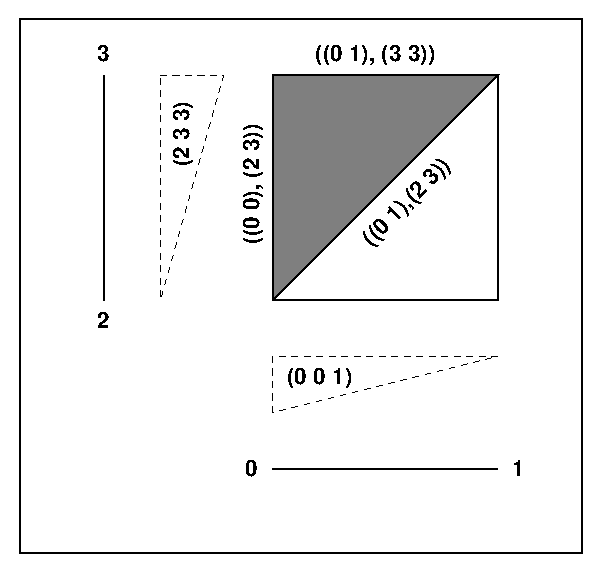
\includegraphics{eml3.eps}}
%
\vskip 0.50cm
{\footnotesize\begin{verbatim}
(? aw-mrp 1 diagonal)  ==>

----------------------------------------------------------------------{CMBN 1}
<1 * <TnPr 0 0 1 2-3>>
<1 * <TnPr 1 0-1 0 3>>
------------------------------------------------------------------------------

(? eml-mrp *)  ==>

----------------------------------------------------------------------{CMBN 1}
<1 * <CrPr - 0-1 0 3>>
<1 * <CrPr 0 0 - 2-3>>
------------------------------------------------------------------------------

(? phi-hmy 1 diagonal)  ==>

----------------------------------------------------------------------{CMBN 2}
<-1 * <CrPr 0 0-1 1 2-3>>
------------------------------------------------------------------------------
\end{verbatim}}
Let us inspect now the reduction generated by the function {\tt ez} and 
verify on reasonably general combinations that the involved morphisms  are coherent.
{\footnotesize\begin{verbatim}
(setf ez-rdc (ez (soft-delta-infinity)(soft-delta-infinity)))  ==>

[K34 Reduction]

(inspect *)  ==>

REDUCTION @ #x36a55a = [K34 Reduction]
   0 Class --------> #<STANDARD-CLASS REDUCTION>
   1 ORGN ---------> <...>, a proper list with 3 elements
   2 IDNM ---------> fixnum 34 [#x00000088]
   3 H ------------> [K33 Morphism (degree 1)]
   4 G ------------> [K11 Morphism (degree 0)]
   5 F ------------> [K12 Morphism (degree 0)]
   6 BCC ----------> [K3 Chain-Complex]
   7 TCC ----------> [K6 Simplicial-Set]
\end{verbatim}}
With the comment slots we see that the morphism {\em f}, {\em g} and {\em h}
are respectively {\em aw}, {\em eml} and {\em phi}:
{\footnotesize\begin{verbatim}
(orgn ez-rdc)  ==>

(EILENBERG-ZILBER [K1 Simplicial-Set][K1 Simplicial-Set])

(orgn (f ez-rdc)) ==>

(AW [K1 Simplicial-Set][K1 Simplicial-Set])

(orgn (g ez-rdc))  ==>

(EML [K1 Simplicial-Set][K1 Simplicial-Set])

(orgn (h ez-rdc))  ==>

(PHI [K1 Simplicial-Set][K1 Simplicial-Set])

(setf *bc* (cmbn 3 1 (tnpr 0 (code '(0)) 3 (code '(1 2 3 4)))
                  10 (tnpr 1 (code '(5 6)) 2 (code '(7 8 9)))
                 100 (tnpr 2 (code '(10 11 12)) 1 (code '(13 14)))
                1000 (tnpr 3 (code '(15 16 17 18)) 0 (code '(19)))))  ==>

----------------------------------------------------------------------{CMBN 3}
<1 * <TnPr 0 1-2-3-4>>
<10 * <TnPr 5-6 7-8-9>>
<100 * <TnPr 10-11-12 13-14>>
<1000 * <TnPr 15-16-17-18 19>>
------------------------------------------------------------------------------
\end{verbatim}}
\newpage
{\footnotesize\begin{verbatim}
(setf *tc* 
     (cmbn 3 1 (crpr 0 (code '(0 1 2 3)) 0 (code '(5 6 7 8)))
            10 (crpr 0 (code '(0 1 2 3)) (dgop-ext-int '(2 0)) (code '(5 6)))
           100 (crpr (dgop-ext-int '(2 1)) (code '(0 1)) 0 (code '(5 6 7 8)))
          1000 (crpr (dgop-ext-int '(2 1)) (code '(0 1)) 1 (code '(5 6 7)))))

----------------------------------------------------------------------{CMBN 3}
<1 * <CrPr - 0-1-2-3 - 5-6-7-8>>
<10 * <CrPr - 0-1-2-3 2-0 5-6>>
<100 * <CrPr 2-1 0-1 - 5-6-7-8>>
<1000 * <CrPr 2-1 0-1 0 5-6-7>>
------------------------------------------------------------------------------

(pre-check-rdct ez-rdc)  ==>

---done---

(check-rdct)  ==>

*TC* => 
----------------------------------------------------------------------{CMBN 3}
<1 * <CrPr - 0-1-2-3 - 5-6-7-8>>
<10 * <CrPr - 0-1-2-3 2-0 5-6>>
<100 * <CrPr 2-1 0-1 - 5-6-7-8>>
<1000 * <CrPr 2-1 0-1 0 5-6-7>>
------------------------------------------------------------------------------

*BC* => 
----------------------------------------------------------------------{CMBN 3}
<1 * <TnPr 0 1-2-3-4>>
<10 * <TnPr 5-6 7-8-9>>
<100 * <TnPr 10-11-12 13-14>>
<1000 * <TnPr 15-16-17-18 19>>
------------------------------------------------------------------------------

Checking *TDD* = 0
Result: 
----------------------------------------------------------------------{CMBN 1}
------------------------------------------------------------------------------

Checking *BDD* = 0
Result: 
----------------------------------------------------------------------{CMBN 1}
------------------------------------------------------------------------------

Checking *DF-FD* = 0
Result: 
----------------------------------------------------------------------{CMBN 2}
------------------------------------------------------------------------------

Checking *DG-GD* = 0
Result: 
----------------------------------------------------------------------{CMBN 2}
------------------------------------------------------------------------------

Checking *ID-FG* = 0
Result: 
----------------------------------------------------------------------{CMBN 3}
------------------------------------------------------------------------------

Checking *ID-GF-DH-HD* = 0
Result: 
----------------------------------------------------------------------{CMBN 3}
------------------------------------------------------------------------------

Checking *HH* = 0
Result: 
----------------------------------------------------------------------{CMBN 5}
------------------------------------------------------------------------------

Checking *FH* = 0
Result: 
----------------------------------------------------------------------{CMBN 4}
------------------------------------------------------------------------------

Checking *HG* = 0
Result: 
----------------------------------------------------------------------{CMBN 4}
------------------------------------------------------------------------------

---done---
\end{verbatim}}

\section {Application to Homology}

Let us  illustrate the Eilenberg-Zilber theorem\index{Eilenberg-Zilber theorem!application of} by the following example. 
Let us consider the manifold $P^2{\R}\times S^3$. The theorem says that
$$H_n({\cal C}_*(P^2{\R}\times S^3)) \cong H_n({\cal C}_*(P^2{\R}) \otimes {\cal C}_*(S^3)).$$
{\footnotesize\begin{verbatim}
(setf p2 (moore 2 1))  ==>      ;; Moore(2,1)   generates the projectif plane.

[K1 Simplicial-Set]

(setf s3 (sphere 3))  ==>

[K6 Simplicial-Set]
\end{verbatim}}
The simplicial set {\tt p2-X-s3} is obtained from the cartesian product of
the two simplicial sets {\tt p2} and {\tt s3}.
{\footnotesize\begin{verbatim}
(setf p2-X-s3 (crts-prdc p2 s3))  ==>

[K11 Simplicial-Set]
\end{verbatim}}
Now, the chain complex {\tt p2-T-s3} is obtained from the tensor product of
the two chain complexes associated to both simplicial sets {\tt p2} and {\tt s3} (don't forget that the class
{\tt SIMPLICIAL SET} is a subclass of the class {\tt CHAIN COMPLEX}).
{\footnotesize\begin{verbatim}
(setf p2-T-s3 (tnsr-prdc p2 s3))  ==>

[K16 Chain-Complex]
\end{verbatim}}
Applying  successively the  function {\tt chcm-homology} (which computes directly the
homology groups without using a homotopy equivalence)  on these chain
complexes, shows that  the homology groups are  effectively isomorphic,
but the method  of the tensor  product is  much faster than the
method of the simple cartesian product, the number of generators being much more 
smaller.
{\footnotesize\begin{verbatim}
(time(dotimes (i 6)(chcm-homology p2-X-s3 i))) ==>

Homology in dimension 0 :

Component Z

Homology in dimension 1 :

Component Z/2Z

Homology in dimension 2 :

Homology in dimension 3 :

Component Z

Homology in dimension 4 :

Component Z/2Z

Homology in dimension 5 :

---done---

; cpu time (non-gc) 880 msec user, 170 msec system
; cpu time (gc)     250 msec user, 0 msec system
; cpu time (total)  1,130 msec user, 170 msec system
; real time  2,563 msec
; space allocation:
;  43,812 cons cells, 64 symbols, 162,904 other bytes

(time(dotimes (i 6)(chcm-homology p2-T-s3 i)))  ==>

Homology in dimension 0 :

Component Z

Homology in dimension 1 :

Component Z/2Z

Homology in dimension 2 :

Homology in dimension 3 :

Component Z

Homology in dimension 4 :

Component Z/2Z

Homology in dimension 5 :

---done---

; cpu time (non-gc) 130 msec user, 20 msec system
; cpu time (gc)     0 msec user, 0 msec system
; cpu time (total)  130 msec user, 20 msec system
; real time  326 msec
; space allocation:
;  1,897 cons cells, 0 symbols, 11,232 other bytes
\end{verbatim}}
The following example shows clearly the discrepancy between the length of
the basis of two  objects built respectively by cartesian product and tensor product and
having the same homology groups.
{\footnotesize\begin{verbatim}
(setf s2 (sphere 2))  ==>

[K1 Simplicial-Set]

(setf s3 (sphere 3))  ==>

[K6 Simplicial-Set]

(setf s2Xs2Xs3 (crts-prdc (crts-prdc s2 s2) s3))  ==>

[K16 Simplicial-Set]

(orgn s2Xs2Xs3)  ==>

(CRTS-PRDC [K23 Simplicial-Set] [K6 Simplicial-Set])

(setf s2Ts2Ts3 (tnsr-prdc (tnsr-prdc s2 s2) s3))   ==>

[K21 Chain-Complex]

(dotimes (i 7) (print(length(basis s2Xs2Xs3 i))))  ==>

1 
0 
3 
22 
138 
390 
480 

(dotimes (i 7) (print(length(basis s2Ts2Ts3 i))))  ==>

1 
0 
2 
1 
1 
2 
0 
\end{verbatim}}

\newpage

\subsection {Searching homology process for cartesian products}

When\index{searching homology!cartesian products} the {\tt search-efhm} method recognizes a cartesian product,
by means of the comment list (slot {\tt orgn}) of the object, it builds a homotopy equivalence where 
the right bottom chain complex is created by the function {\tt ez}. 
The process may be recursif as shown by the very definition of the method:
\vskip 0.35cm
{\footnotesize\begin{verbatim}
(defun LEFT-CRTS-PRDC-EFHM (smst1 smst2)
  (declare (type simplicial-set smst1 smst2))
  (the homotopy-equivalence
     (build-hmeq
       :lrdct (trivial-rdct (crts-prdc smst1 smst2))
       :rrdct (ez smst1 smst2))))

(defmethod SEARCH-EFHM (smst (orgn (eql 'crts-prdc)))
  (declare (type simplicial-set smst))
  (the homotopy-equivalence
    (cmps
      (left-crts-prdc-efhm (second (orgn smst)) 
                           (third  (orgn smst)))
      (tnsr-prdc (efhm (second (orgn smst)))
                 (efhm (third  (orgn smst)))))))
\end{verbatim}}

\subsection* {Lisp files concerned in this chapter}

{\tt eilenberg-zilber.lisp}, {\tt searching-homology.lisp}.

